\documentclass[12pt,a4paper]{report}

% ===================== PACKAGES =====================
\usepackage[utf8]{inputenc}
\usepackage[T1]{fontenc}
\usepackage[french]{babel}
\usepackage{lmodern}
\usepackage{geometry}
\geometry{a4paper, left=2.5cm, right=2.5cm, top=2.5cm, bottom=2.5cm}
\usepackage{graphicx}
\usepackage{float}
\usepackage{amsmath, amssymb}
\usepackage{listings}
\usepackage{xcolor}
\usepackage{booktabs}
\usepackage{hyperref}
\hypersetup{
    colorlinks=true,
    linkcolor=black,
    citecolor=black,
    urlcolor=blue,
    pdftitle={Monographie - MedBox AI},
}
\usepackage{fancyhdr}
\usepackage{titlesec}
\usepackage{setspace}
\onehalfspacing

% ===================== CONFIG CODE (LISTINGS) =====================
\lstset{
    basicstyle=\ttfamily\small,
    breaklines=true,
    frame=single,
    backgroundcolor=\color{gray!10},
    numbers=left,
    numberstyle=\tiny,
    keywordstyle=\color{blue},
    commentstyle=\color{gray},
}

% ===================== EN-TETES =====================
\setlength{\headheight}{14pt}
\pagestyle{fancy}
\fancyhf{}
\fancyhead[L]{\leftmark}
\fancyfoot[C]{\thepage}
\renewcommand{\headrulewidth}{0.4pt}

% ===================== INFOS A COMPLETER =====================
\newcommand{\titreProjet}{MedBox AI}
\newcommand{\sousTitre}{Boîtier de diagnostic médical embarqué basé sur l'intelligence artificielle}
\newcommand{\nomEtudiant}{BIDIKI Enock}
\newcommand{\nomEtablissement}{Université Protestante au Congo}
\newcommand{\nomFaculte}{Faculté des Sciences Informatiques}
\newcommand{\nomFormation}{Licence 2 -- LMD}
\newcommand{\anneeUniv}{Année académique 2025 -- 2026}

\begin{document}

% ===================== PAGE DE TITRE =====================
\begin{titlepage}
    \centering
    {\scshape\Large \nomEtablissement \par}
    {\scshape \nomFaculte \par}
    {\scshape \nomFormation \par}
    \vspace{2cm}

    {\huge\bfseries Monographie \par}
    \vspace{1cm}
    \rule{\linewidth}{0.5mm} \\[0.4cm]
    {\Huge \titreProjet \par}
    {\large \sousTitre \par}
    \rule{\linewidth}{0.5mm} \\[1.5cm]

    \begin{minipage}{0.45\textwidth}
        \begin{center} \large
            \textit{Réalisé par :}\\
            \nomEtudiant
        \end{center}
    \end{minipage}
    \vfill
    {\large \anneeUniv \par}
\end{titlepage}

% ===================== RESUME =====================
\chapter*{Résumé}
\addcontentsline{toc}{chapter}{Résumé}

Ce projet de monographie s'inscrit dans le cadre de l'initiation à la démarche scientifique et à l'ingénierie embarquée au sein de la Faculté des Sciences Informatiques. Il porte sur la conception d'un boîtier médical autonome, nommé MedBox AI, capable de mesurer automatiquement plusieurs constantes vitales d'un patient et de proposer localement un diagnostic parmi dix-neuf profils physiologiques et pathologiques, à l'aide d'un modèle d'intelligence artificielle embarqué sur un microcontrôleur. L'approche suivie combine la constitution d'un jeu de données médicales, l'entraînement d'un réseau de neurones de classification, la conversion de ce modèle pour une exécution locale sur microcontrôleur, ainsi que la conception d'un système électronique intégrant plusieurs capteurs biométriques et un module d'identification par carte à puce sans contact. Les résultats obtenus démontrent la faisabilité d'un diagnostic médical préliminaire entièrement autonome et sans connexion réseau, tout en révélant plusieurs limites techniques inhérentes à un prototype construit avec des composants grand public. Ce travail illustre ainsi la capacité de l'étudiant à mobiliser des compétences pluridisciplinaires, allant de l'intelligence artificielle à l'électronique embarquée, pour concevoir un système fonctionnel répondant à une problématique concrète.

% ===================== SOMMAIRE =====================
\tableofcontents
\clearpage

% ===================== CHAPITRE 1 : INTRODUCTION GENERALE =====================
\chapter{Introduction générale}

\section{Contexte}
L'accès à un premier diagnostic médical fiable et rapide reste un enjeu majeur, en particulier dans les contextes où le personnel soignant est peu disponible ou éloigné (zones rurales, postes de secours, dépistage de masse). Les objets connectés couplés à l'intelligence artificielle embarquée, communément désignée par le terme \textit{TinyML}, offrent aujourd'hui une réponse crédible à cette problématique : ils permettent de réaliser une analyse médicale préliminaire directement sur un microcontrôleur, sans connexion internet ni serveur distant. C'est dans cette optique que s'inscrit le projet MedBox AI, un boîtier autonome construit autour d'un microcontrôleur ESP32, capable de mesurer plusieurs constantes vitales d'un patient et d'exécuter localement un modèle d'intelligence artificielle pour proposer un diagnostic.

\section{Problématique}
La problématique centrale du projet peut être formulée ainsi : comment concevoir un système embarqué, autonome et peu coûteux, capable de mesurer automatiquement les constantes vitales d'un patient et d'en déduire, localement et en temps réel, un diagnostic parmi un ensemble de profils physiologiques et pathologiques courants, tout en restant réalisable avec des composants électroniques grand public et des bibliothèques logicielles ouvertes ?

\subsection*{Sous-questions techniques}
\begin{itemize}
    \item Quelles grandeurs physiologiques mesurer, et avec quels capteurs, pour obtenir une donnée exploitable par un modèle d'intelligence artificielle ?
    \item Comment entraîner un modèle de classification suffisamment précis tout en restant assez léger pour tenir dans la mémoire limitée d'un microcontrôleur ?
    \item Comment garantir la fiabilité des mesures issues de capteurs bas coût, sujettes au bruit et aux artefacts de mouvement ?
    \item Comment organiser le déroulement logiciel (acquisition, traitement, inférence, affichage) de manière robuste, malgré les contraintes matérielles du microcontrôleur ?
\end{itemize}

\section{Objectifs}

\subsection{Objectif général}
Concevoir et réaliser un prototype de boîtier médical embarqué, autonome et fonctionnel, capable de mesurer les constantes vitales d'un patient et de fournir localement un diagnostic à l'aide d'un modèle d'intelligence artificielle, en mobilisant les compétences acquises en programmation, en électronique embarquée et en apprentissage automatique.

\subsection{Objectifs spécifiques}
\begin{itemize}
    \item Concevoir un boîtier matériel intégrant les capteurs nécessaires à la mesure de quatre grandeurs : âge, fréquence cardiaque, saturation en oxygène et température corporelle.
    \item Constituer un jeu de données représentatif de dix-neuf profils physiologiques et pathologiques, puis entraîner un modèle de classification multiclasse.
    \item Convertir ce modèle au format TensorFlow Lite et l'embarquer sur le microcontrôleur pour une inférence entièrement locale.
    \item Développer une machine à états gérant l'identification du patient, l'acquisition des capteurs, l'inférence de l'intelligence artificielle et l'affichage du résultat.
    \item Identifier, documenter et corriger les dysfonctionnements rencontrés lors de l'intégration matérielle et logicielle.
    \item Évaluer les performances et les limites du système à travers des tests, tant en simulation qu'avec le matériel réel.
\end{itemize}

\section{Méthodologie adoptée}
Le travail s'est déroulé en plusieurs étapes successives. L'étudiant a d'abord mené une analyse du besoin et une recherche des composants électroniques adaptés. Il a ensuite procédé à la constitution d'un jeu de données et à l'entraînement d'un modèle d'intelligence artificielle sous Python, avant de convertir ce modèle pour une exécution embarquée. La phase suivante a consisté en l'implémentation pratique du firmware sur microcontrôleur ESP32, organisée en modules logiciels indépendants (capteurs, identification, intelligence artificielle, affichage). Des tests répétés, en simulation puis avec les capteurs physiques, ont permis de détecter et corriger plusieurs dysfonctionnements. Tout au long du processus, l'étudiant a été encadré par un enseignant référent.

\section{Structure du document}
Ce document est structuré en cinq chapitres principaux. Le premier chapitre, \textit{Introduction générale}, présente le contexte, la problématique, les objectifs, la méthodologie et l'organisation du travail. Le deuxième chapitre, \textit{Cadre théorique et technologique}, définit les concepts clés mobilisés et décrit les outils et technologies utilisés. Le troisième chapitre, \textit{Réalisation du projet}, présente les étapes concrètes du développement de la solution. Le quatrième chapitre, \textit{Difficultés rencontrées et limites}, expose les contraintes techniques rencontrées et les limites observées du prototype. Enfin, le cinquième chapitre, \textit{Conclusion générale}, récapitule le travail effectué, présente les apports du projet et propose des perspectives d'amélioration.

% ===================== CHAPITRE 2 : CADRE THEORIQUE ET TECHNOLOGIQUE =====================
\chapter{Cadre théorique et technologique}

\section{Définitions des concepts clés}

\textbf{Intelligence artificielle embarquée (TinyML).} Sous-domaine de l'apprentissage automatique consistant à déployer des modèles d'intelligence artificielle directement sur des microcontrôleurs à ressources très limitées (quelques kilo-octets à quelques mégaoctets de mémoire), sans dépendre d'un serveur distant. Cette approche est au cœur de MedBox AI, dont le modèle de diagnostic s'exécute entièrement sur l'ESP32.

\textbf{Réseau de neurones de type Perceptron Multicouche (MLP).} Modèle d'apprentissage automatique composé de plusieurs couches de neurones artificiels interconnectées, capable d'apprendre à classer des données à partir d'exemples. Dans ce projet, un MLP est utilisé pour classer les mesures d'un patient parmi dix-neuf profils physiologiques et pathologiques.

\textbf{Normalisation Z-score.} Technique de mise à l'échelle des données consistant à soustraire la moyenne et diviser par l'écart-type de chaque variable, afin que toutes les variables d'entrée du modèle aient une échelle comparable. Cette étape est indispensable pour la stabilité de l'apprentissage d'un réseau de neurones.

\textbf{Quantification de modèle.} Processus de compression d'un modèle d'intelligence artificielle consistant à réduire la précision numérique de ses paramètres, afin de diminuer sa taille en mémoire et d'accélérer son exécution sur un matériel aux ressources limitées.

\textbf{Communication I2C.} Protocole de communication série permettant à plusieurs composants électroniques (capteurs, écran, module de communication) de dialoguer avec un microcontrôleur sur un même bus, en utilisant seulement deux fils.

\textbf{Photopléthysmographie.} Technique de mesure optique consistant à éclairer la peau (généralement le doigt) avec une lumière infrarouge et rouge, puis à analyser la lumière réfléchie pour en déduire la fréquence cardiaque et la saturation en oxygène du sang.

\textbf{Communication en champ proche (NFC).} Technologie de communication sans fil à très courte portée, utilisée dans ce projet pour lire l'âge d'un patient stocké sur un badge, via un module dédié.

\section{Présentation des outils ou technologies utilisés}

\begin{itemize}
    \item \textbf{ESP32} : microcontrôleur central du projet, choisi pour sa puissance de calcul suffisante, son faible coût et sa capacité à exécuter des modèles d'intelligence artificielle allégés. Il pilote l'ensemble des périphériques et exécute le firmware complet.
    \item \textbf{MAX30102} (bibliothèque SparkFun) : capteur optique de photopléthysmographie permettant de mesurer la fréquence cardiaque et la saturation en oxygène. Choisi pour son faible coût et sa large documentation communautaire.
    \item \textbf{MLX90614} (bibliothèque Adafruit) : capteur infrarouge sans contact permettant de mesurer la température corporelle du patient sans contact direct, pour des raisons d'hygiène.
    \item \textbf{PN532} (bibliothèque Adafruit) : module de lecture NFC utilisé pour identifier le patient et extraire son âge depuis un badge.
    \item \textbf{Écran OLED SSD1306} : afficheur utilisé pour présenter les mesures en temps réel puis le diagnostic final à l'utilisateur.
    \item \textbf{Python, avec les bibliothèques pandas, scikit-learn et TensorFlow/Keras} : environnement utilisé pour préparer le jeu de données, entraîner le modèle de classification et le convertir au format embarqué.
    \item \textbf{TensorFlow Lite for Microcontrollers} (via les bibliothèques \texttt{tflm\_esp32} et \texttt{eloquent\_tinyml}) : cadriciel permettant d'exécuter le modèle d'intelligence artificielle quantifié directement sur l'ESP32.
    \item \textbf{Arduino IDE / C++} : environnement de développement utilisé pour écrire, compiler et téléverser le firmware embarqué sur l'ESP32.
    \item \textbf{Microsoft Excel} : utilisé pour la constitution et l'organisation du jeu de données de 9500 échantillons ayant servi à l'entraînement du modèle.
\end{itemize}

% ===================== CHAPITRE 3 : REALISATION DU PROJET =====================
\chapter{Réalisation du projet}

\section{Analyse des besoins}
Le système devait répondre aux besoins fonctionnels suivants :
\begin{itemize}
    \item Identifier un patient de manière simple et rapide, sans saisie manuelle.
    \item Mesurer automatiquement, sans intervention d'un professionnel de santé, quatre grandeurs physiologiques : âge, fréquence cardiaque, saturation en oxygène et température corporelle.
    \item Traiter ces données localement pour produire un diagnostic parmi dix-neuf profils possibles, sans dépendre d'une connexion internet.
    \item Afficher un résultat clair et lisible à l'utilisateur.
\end{itemize}

Ces besoins fonctionnels s'accompagnaient de contraintes non fonctionnelles fortes, propres à l'embarqué : mémoire vive très limitée (quelques centaines de kilo-octets), nécessité d'un fonctionnement autonome (sans serveur), et budget matériel restreint imposant l'usage de capteurs grand public plutôt que de dispositifs médicaux certifiés.

\section{Architecture de la solution}
Le boîtier MedBox AI repose sur un microcontrôleur ESP32 connecté en bus I2C à l'ensemble des périphériques. L'architecture logicielle est organisée en modules indépendants, chacun responsable d'un sous-système :

\begin{itemize}
    \item \texttt{config.h} : définition des états de la machine, de la structure de données patient, des constantes de normalisation et de calibration.
    \item \texttt{nfc\_module.h} : gestion de l'identification du patient via le module PN532.
    \item \texttt{sensors\_module.h} : gestion de l'acquisition des mesures physiologiques (MAX30102, MLX90614).
    \item \texttt{ia\_inference.h} : normalisation des données et exécution de l'inférence TensorFlow Lite Micro.
    \item \texttt{display\_module.h} : gestion de l'affichage sur l'écran OLED.
\end{itemize}

Le fonctionnement global est piloté par une \textbf{machine à états finis}, qui structure le cycle de vie complet d'une mesure patient :

\begin{enumerate}
    \item \texttt{STATE\_WAIT\_NFC} : attente du scan d'un badge NFC, permettant d'extraire l'âge du patient.
    \item \texttt{STATE\_READ\_SENSORS} : acquisition de la température (détection de présence), puis de la fréquence cardiaque et de la saturation en oxygène.
    \item \texttt{STATE\_SCALING} : normalisation Z-score des quatre variables mesurées.
    \item \texttt{STATE\_INFERENCE} : exécution de l'inférence TinyML locale.
    \item \texttt{STATE\_SHOW\_RESULT} : affichage du diagnostic pendant dix secondes, avant réinitialisation pour un nouveau patient.
\end{enumerate}

\begin{figure}[H]
    \centering
    % \includegraphics[width=0.7\textwidth]{schema_architecture.png}
    \caption{Schéma de l'architecture matérielle et logicielle de MedBox AI}
    \label{fig:architecture}
\end{figure}

\section{Étapes de mise en œuvre}

\subsection*{Phase de conception}
Le projet a débuté par la définition des dix-neuf profils physiologiques et pathologiques à reconnaître (états normaux selon l'âge, variations physiologiques légères, et pathologies de sévérité croissante telles que tachycardie, bradycardie, hypoxie, fièvre ou choc). Les seuils retenus pour chaque classe (plages de fréquence cardiaque, de saturation en oxygène et de température selon l'âge) ont été construits à partir de tables de référence clinique reconnues, notamment le Manuel MSD, les directives \textit{Pediatric Advanced Life Support} de l'American Heart Association pour les seuils pédiatriques, ainsi que les repères cliniques de détresse et de choc publiés par l'Organisation mondiale de la santé.

Un jeu de données synthétique de 9500 échantillons a ensuite été constitué, parfaitement équilibré entre les dix-neuf classes (500 échantillons par classe), avec pour chaque échantillon quatre variables d'entrée (âge, fréquence cardiaque, saturation en oxygène, température) et une étiquette de classe. Le recours à des données synthétiques plutôt qu'à des données patients réelles se justifie à la fois sur le plan éthique et sur le plan pratique : les principes relatifs aux données de l'Organisation mondiale de la santé rappellent qu'aucune donnée réelle de patient ne doit être utilisée sans infrastructure de protection et d'anonymisation adaptée, hors de portée d'un projet étudiant. Sur le plan scientifique, la littérature reconnaît par ailleurs l'usage de données synthétiques comme une pratique validée en santé numérique, en particulier pour l'éducation, la formation et le développement de logiciels de santé, ainsi que pour tester des algorithmes et générer des hypothèses avant toute manipulation de données réelles.

\subsection*{Phase d'implémentation}

\paragraph{Entraînement du modèle d'intelligence artificielle.} Un réseau de neurones de type Perceptron Multicouche a été entraîné sous Python/Keras, avec l'architecture suivante : une couche d'entrée à 4 neurones, une première couche cachée de 32 neurones (activation ReLU), une couche de régularisation (Dropout à 10~\%), une seconde couche cachée de 16 neurones (activation ReLU), et une couche de sortie de 19 neurones (activation Softmax). L'entraînement a été réalisé avec l'optimiseur Adam, une fonction de perte de type \textit{categorical crossentropy}, sur 50 itérations complètes (\textit{epochs}) et des lots de 32 échantillons, sur un ensemble d'entraînement représentant 80~\% du jeu de données (les 20~\% restants formant l'ensemble de test).

\paragraph{Conversion pour l'embarqué.} Le modèle entraîné a ensuite été converti au format TensorFlow Lite avec quantification par défaut, afin de réduire sa taille et d'accélérer son exécution sur microcontrôleur. Le fichier obtenu a été transformé en tableau d'octets C++, directement intégrable dans le firmware. Sur l'ESP32, l'inférence est exécutée avec une zone mémoire de seulement 8~kilo-octets de SRAM, illustrant la légèreté du modèle final.

\paragraph{Développement du firmware embarqué.} Le firmware a été développé en C++ sous Arduino IDE, avec la structure modulaire décrite en section 3.2. Un mode de simulation a été ajouté à deux niveaux du système : un mode de simulation NFC (badge simulé par une valeur d'âge fixe dans le code) et un mode de saisie manuelle des constantes vitales via le moniteur série, permettant de tester les dix-neuf classes de sortie du modèle sans avoir à reproduire physiquement chaque état pathologique avec les capteurs.

\subsection*{Phase de tests}
Les tests ont été menés à deux niveaux. D'une part, le modèle a été évalué automatiquement sur l'ensemble de test Python (1900 échantillons non vus pendant l'entraînement). D'autre part, le prototype matériel complet a été testé de manière itérative, ce qui a permis de mettre en évidence plusieurs dysfonctionnements (détaillés au chapitre 4) et d'orienter les corrections successives apportées au firmware, notamment sur la fiabilité de la mesure cardiaque et sur la lecture des badges NFC.

\section{Résultats obtenus}

\subsection*{Performance du modèle d'intelligence artificielle}
Après entraînement, le modèle atteint une précision de \textbf{95,58~\%} sur l'ensemble de test. Cette précision est quasiment intégralement préservée après conversion et quantification au format TensorFlow Lite, confirmant que la compression du modèle n'a pas dégradé significativement ses performances.

\begin{figure}[H]
    \centering
    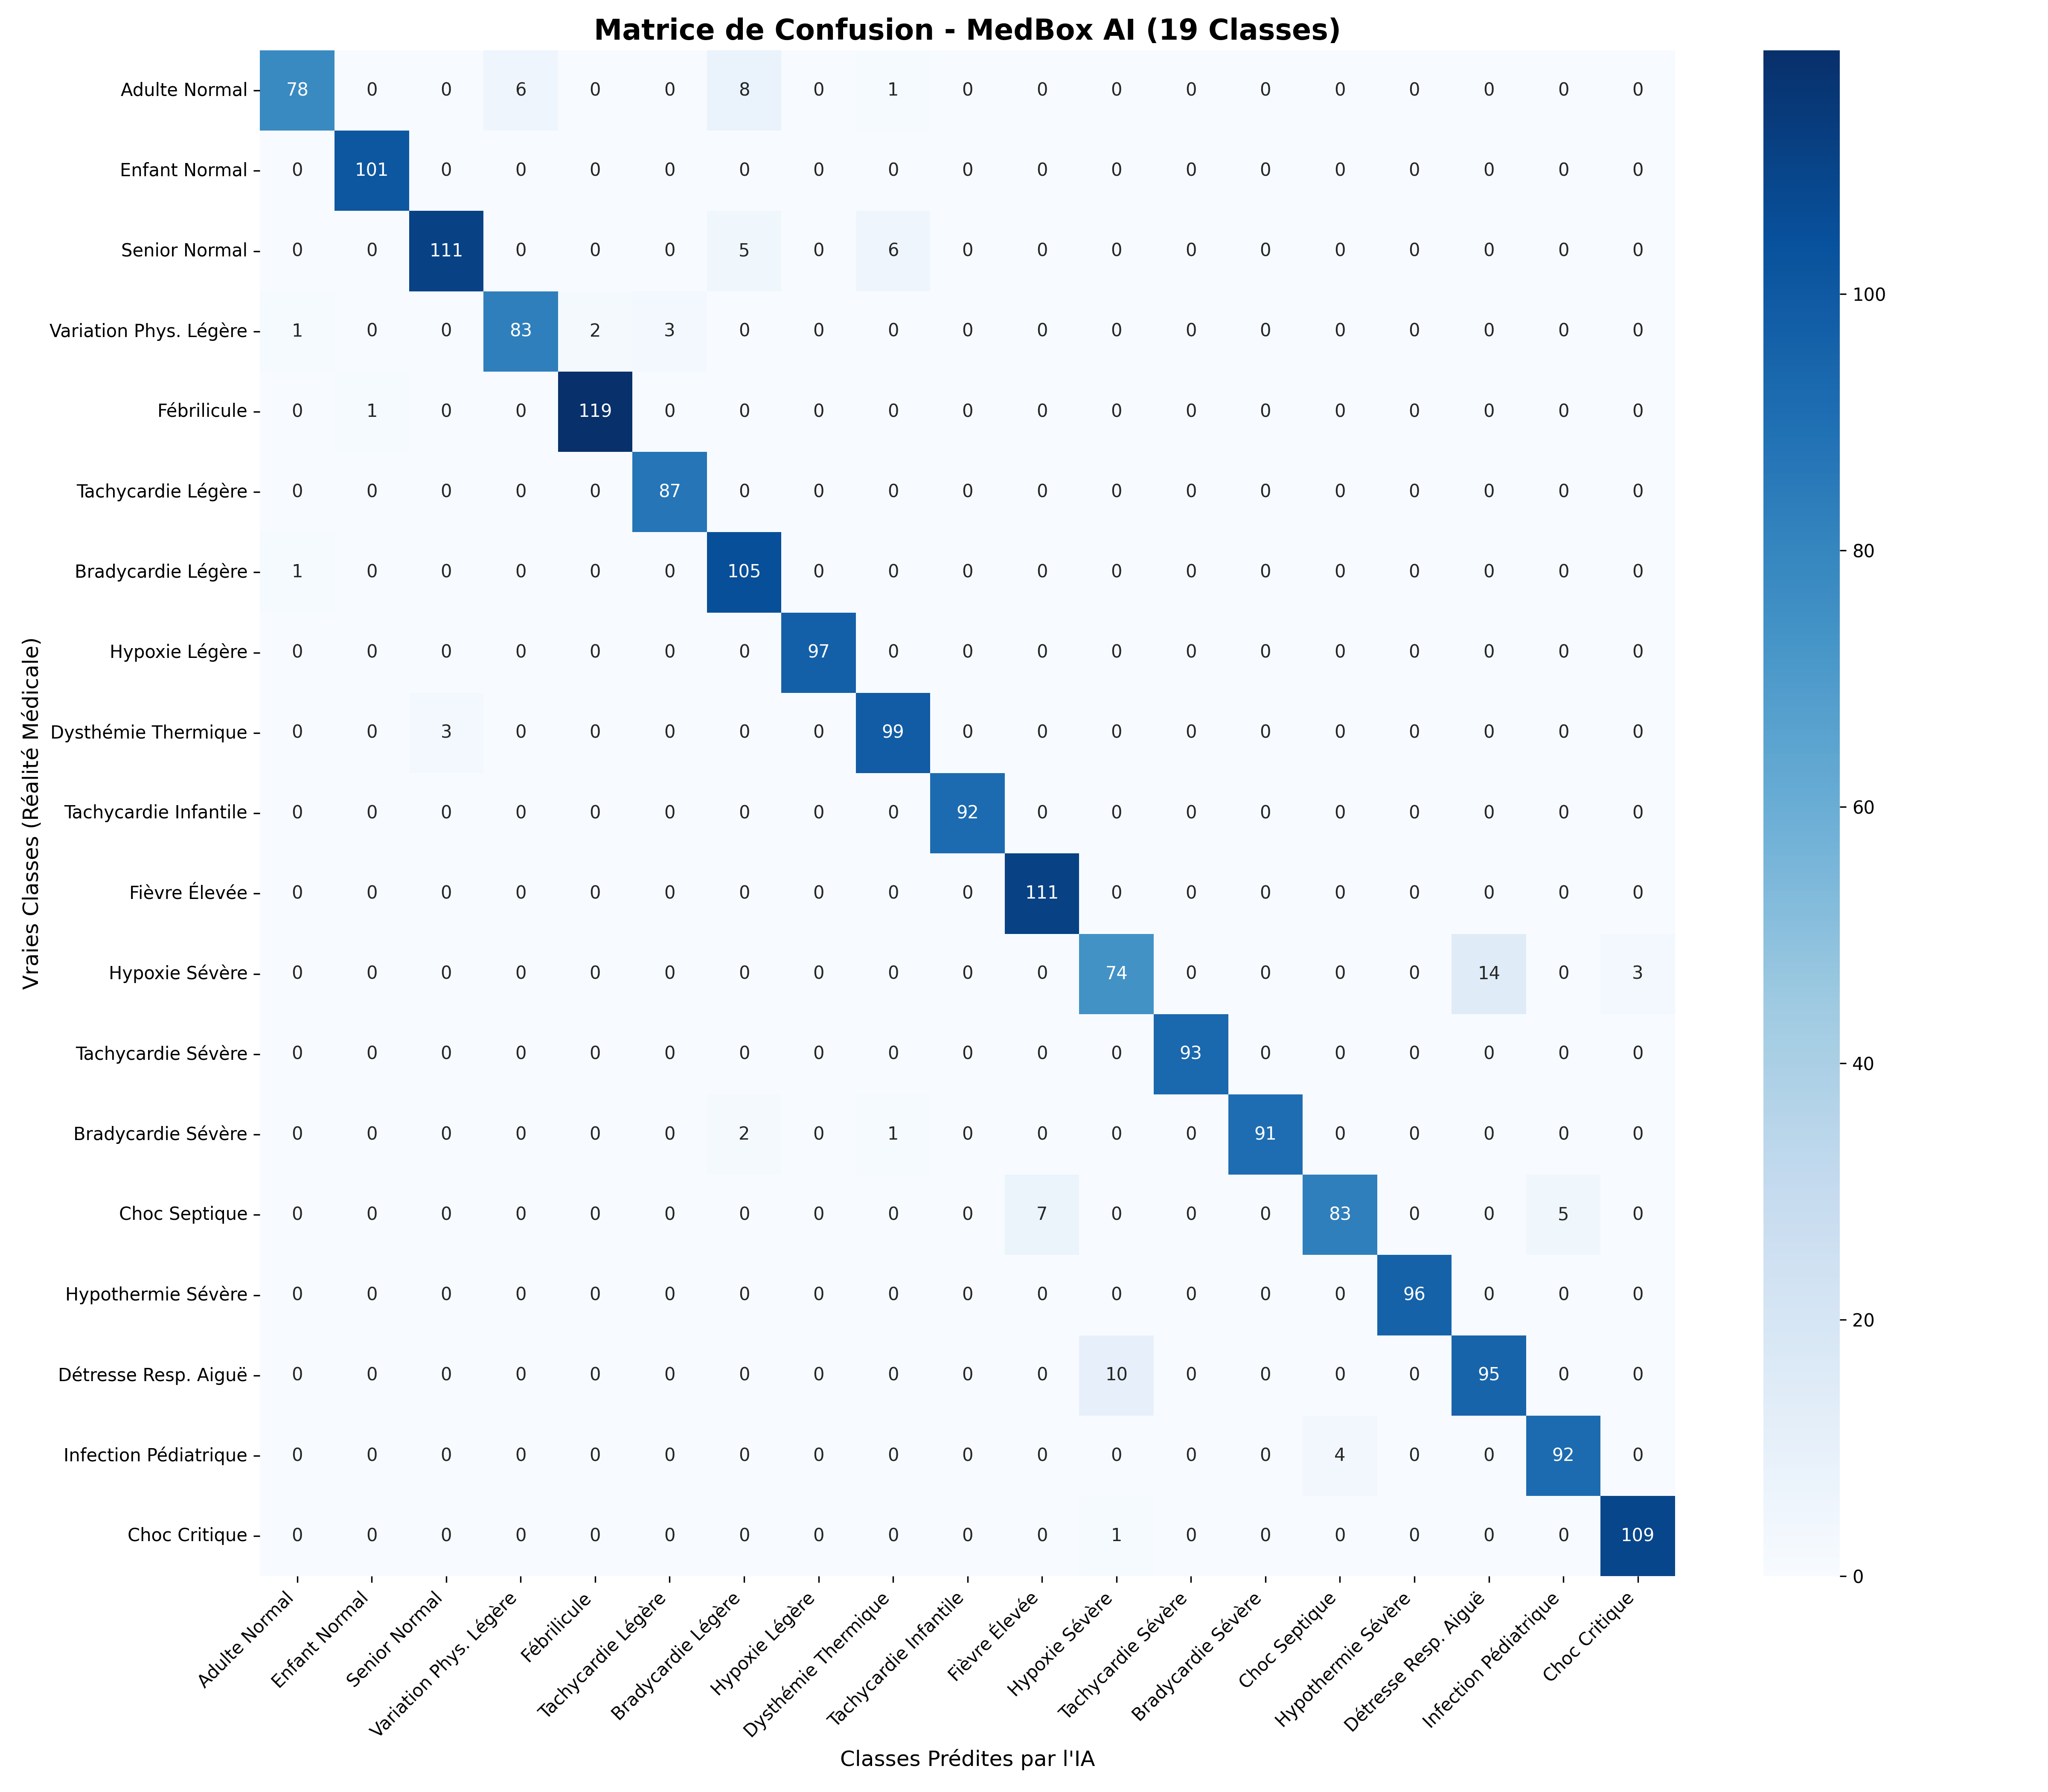
\includegraphics[width=0.95\textwidth]{matrice_confusion_medbox.png}
    \caption{Matrice de confusion du modèle MedBox AI sur les 19 classes}
    \label{fig:confusion}
\end{figure}

L'analyse de la matrice de confusion (figure~\ref{fig:confusion}) montre que la quasi-totalité des classes sont très bien reconnues. Les rares confusions observées concernent presque exclusivement des classes physiologiquement proches, par exemple \textit{Adulte Normal} confondu occasionnellement avec \textit{Variation Physiologique Légère} ou \textit{Tachycardie Légère}, ou encore \textit{Hypoxie Sévère} confondue avec \textit{Infection Pédiatrique Grave} — des états graves partageant des profils de constantes vitales proches. Ces confusions restent limitées et concentrées sur des cas cliniquement voisins, ce qui confirme la pertinence du modèle pour un usage de premier tri, tout en soulignant qu'il ne saurait remplacer un diagnostic médical complet.

\subsection*{Résultats du prototype matériel}
Une fois le firmware corrigé (voir chapitre 4), le boîtier fonctionne de bout en bout : lecture d'un badge NFC, mesure de la température par calibration empirique, mesure de la fréquence cardiaque et de la saturation en oxygène par cycles successifs, puis inférence et affichage du diagnostic. La calibration du capteur de température, réalisée à partir de huit mesures comparatives avec un thermomètre de référence, a permis de déterminer un offset moyen de correction de +3,98~°C (écart-type des écarts individuels de 0,83~°C), rendant les températures transmises au modèle cohérentes avec la température corporelle réelle. Concernant la mesure cardiaque, des essais répétés sur un même sujet au repos ont révélé une variabilité significative des valeurs retenues (de 83 à 166 battements par minute selon les essais), reflétant les limites du capteur bas coût utilisé plutôt qu'un défaut de la chaîne logicielle de traitement.

% ===================== CHAPITRE 4 : DIFFICULTES ET LIMITES =====================
\chapter{Difficultés rencontrées et limites}

\section{Difficultés rencontrées}
Plusieurs dysfonctionnements techniques ont été identifiés et corrigés au cours du développement du prototype. Ce chapitre les documente de manière transparente, dans un souci d'honnêteté scientifique.

\paragraph{Authentification manquante en lecture NFC.} La fonction de lecture des badges Mifare Classic appelait la lecture d'un bloc mémoire sans authentification préalable du secteur, alors qu'une carte Mifare Classic exige cette authentification avant toute lecture. La lecture échouait donc silencieusement et le système retombait systématiquement sur une valeur d'âge de secours. Correction apportée : ajout de l'authentification par clé par défaut avant chaque lecture du bloc concerné.

\paragraph{Incohérence de format entre écriture et lecture NFC.} Le script d'écriture initial stockait l'âge en texte, alors que la logique de lecture interprétait le premier octet comme une valeur numérique brute, produisant des âges erronés en sortie. Correction apportée : alignement du format d'écriture sur le format brut attendu en lecture.

\paragraph{Calibration insuffisante du capteur de température.} Le capteur infrarouge sans contact mesure la température de peau, systématiquement inférieure de plusieurs degrés à la température corporelle centrale. Sans correction, l'entrée transmise à l'intelligence artificielle restait proche de 32-33~°C, provoquant une classification systématique en « hypothermie sévère ». Correction apportée : calibration empirique à partir de huit mesures comparatives, avec un offset moyen de +3,98~°C appliqué uniquement à la valeur transmise à l'IA et à l'affichage.

\paragraph{Absence de retour visuel après le scan du badge.} Après un scan réussi, l'écran restait figé sur l'écran d'attente jusqu'à la fin complète de la mesure des capteurs. Correction apportée : ajout d'un écran de confirmation intermédiaire (âge lu et signal sonore).

\paragraph{Crash mémoire lors de l'agrandissement de la fenêtre de capture cardiaque.} Une tentative d'agrandir la fenêtre de capture du capteur cardiaque (de 100 à 400 échantillons), pour tenter de stabiliser le calcul du rythme cardiaque, a provoqué un incident critique (\textit{Guru Meditation Error}). La cause identifiée est que la bibliothèque de calcul utilisée repose sur des tableaux de travail internes de taille fixe, codée en dur à 100 échantillons, indépendamment du paramètre transmis. Dépasser cette limite provoque une écriture hors des zones mémoire allouées. Correction apportée : retour à une fenêtre de 100 échantillons (contrainte non modifiable sans réécrire la bibliothèque), compensée par la multiplication du nombre de cycles de mesure indépendants (passé de 1 à 5).

\paragraph{Contention du bus I2C pendant la capture cardiaque.} L'écran OLED et le capteur cardiaque partageant le même bus I2C, le rafraîchissement de l'écran pendant la capture bloquait le bus 20 à 30 millisecondes à chaque appel, perturbant la régularité temporelle du signal nécessaire au calcul fiable du rythme cardiaque. Correction apportée : suppression des mises à jour d'écran pendant la capture, l'affichage n'étant désormais rafraîchi qu'une seule fois au début de chaque cycle de mesure.

\paragraph{Instabilité persistante des mesures cardiaques.} Malgré les corrections précédentes, des valeurs physiologiquement improbables ont continué à apparaître ponctuellement, en particulier lors de micro-mouvements du doigt. Plusieurs corrections cumulatives ont été apportées : renforcement du lissage matériel, multiplication des cycles de mesure indépendants, filtrage des valeurs hors plage physiologique plausible (fréquence cardiaque entre 40 et 200 battements par minute, saturation entre 70 et 100~\%), calcul de la médiane des cycles valides plutôt qu'une moyenne, et ajout d'un garde-fou détectant les cas de doublement de fréquence (phénomène harmonique connu de l'algorithme de calcul), avec préférence donnée à la fréquence fondamentale la plus basse.

\paragraph{Séparation du firmware d'écriture des badges.} L'écriture et la lecture des badges NFC ne pouvant cohabiter dans un même programme exécuté par le microcontrôleur, un programme indépendant a dû être développé spécifiquement pour la préparation des badges, nécessitant un changement de programme téléversé à chaque modification de badge.

\section{Limites de la solution}

\begin{itemize}
    \item \textbf{Précision de la mesure de température.} L'offset de calibration repose sur seulement huit mesures comparatives réalisées sur un nombre restreint de sujets. La marge d'erreur réaliste à attendre en usage reste supérieure à celle d'un thermomètre médical certifié ; cette calibration est indicative et n'a pas été validée cliniquement.
    \item \textbf{Fiabilité du capteur cardiaque.} Même après filtrage, cycles multiples et calcul par médiane, des écarts de mesure significatifs ont été observés sur une même personne au repos. Cette variabilité reflète une limite réelle du capteur bas coût utilisé et de l'algorithme de démonstration associé, qui n'intègrent pas les techniques de rejet de mouvement des oxymètres de pouls commerciaux certifiés.
    \item \textbf{Absence de validation clinique.} Ni les capteurs, ni le modèle de classification, ni les seuils de décision utilisés n'ont été validés par du personnel médical qualifié ni comparés à des dispositifs certifiés. MedBox AI reste un prototype éducatif et ne doit en aucun cas être utilisé comme outil de diagnostic réel.
    \item \textbf{Dépendance au mode de simulation.} Le paramètre de simulation NFC doit être explicitement désactivé pour un usage avec de véritables badges. Un oubli à ce niveau fausserait silencieusement les résultats, sans message d'erreur explicite à l'utilisateur.
    \item \textbf{Couverture de test incomplète du modèle.} La validation des dix-neuf classes de sortie repose majoritairement sur le mode de saisie manuelle des constantes vitales, faute de pouvoir reproduire physiquement chaque état critique avec les capteurs disponibles. La performance du modèle sur des données de capteurs réelles pour ces classes critiques reste donc partiellement non vérifiée.
    \item \textbf{Contrainte matérielle non résolue.} La fenêtre de capture du signal cardiaque, imposée par la bibliothèque de calcul utilisée, n'a pas pu être allongée sans provoquer un crash mémoire. Une fenêtre plus longue améliorerait probablement la stabilité du calcul, mais nécessiterait de réécrire l'algorithme de traitement du signal, ce qui n'a pas été réalisé dans le cadre de ce projet.
\end{itemize}

% ===================== CHAPITRE 5 : CONCLUSION GENERALE =====================
\chapter{Conclusion générale}

\section{Récapitulatif}
Ce projet a porté sur la conception d'un boîtier médical embarqué autonome, MedBox AI, combinant capteurs biométriques, identification par badge NFC et intelligence artificielle embarquée. La démarche suivie a consisté à constituer un jeu de données de 9500 échantillons répartis en dix-neuf profils physiologiques et pathologiques, à entraîner un modèle de classification atteignant 95,58~\% de précision, puis à convertir et intégrer ce modèle sur un microcontrôleur ESP32 via TensorFlow Lite Micro. Le firmware embarqué, organisé autour d'une machine à états, a été développé, testé et corrigé de manière itérative pour aboutir à un prototype fonctionnel.

\section{Apports du projet}
Ce travail a permis à l'étudiant de mobiliser et de développer des compétences pluridisciplinaires : préparation et exploitation d'un jeu de données, entraînement et évaluation d'un modèle d'apprentissage automatique, conversion de modèles pour l'embarqué, programmation en C++ sur microcontrôleur, intégration de capteurs électroniques hétérogènes sur un même bus de communication, et démarche rigoureuse de diagnostic et de correction de dysfonctionnements matériels et logiciels. Le projet a également permis d'appréhender concrètement l'écart, souvent sous-estimé, entre un modèle d'intelligence artificielle performant en simulation et son comportement une fois confronté aux contraintes réelles d'un système embarqué et de capteurs physiques imparfaits.

\section{Perspectives}
Plusieurs perspectives d'amélioration se dégagent de ce travail. L'enrichissement du jeu de données avec des mesures réelles, et non uniquement synthétiques, permettrait de renforcer la robustesse du modèle en conditions réelles. Le remplacement ou la réécriture de l'algorithme de traitement du signal cardiaque permettrait de dépasser la contrainte actuelle de la fenêtre de capture. Une calibration du capteur de température sur un échantillon plus large de sujets renforcerait la fiabilité de cette mesure. Enfin, le développement d'une application mobile ou d'une historisation des résultats, ainsi qu'une validation par du personnel médical qualifié, constitueraient des étapes naturelles vers un dispositif plus abouti, dans la continuité d'un futur mémoire ou projet de fin de cycle.

% ===================== CHAPITRE 6 : BIBLIOGRAPHIE ET WEBOGRAPHIE =====================
\chapter{Bibliographie et Webographie}

\section*{Bibliographie}
\addcontentsline{toc}{section}{Bibliographie}

\subsection*{Justification du recours à des données synthétiques}
\begin{itemize}
    \item Gonzales, A., Guruswamy, G., Smith, S. R. \textit{Synthetic data in health care: A narrative review}. PLOS Digital Health. 2023;2(1):e0000082. doi: 10.1371/journal.pdig.0000082. Disponible sur : \url{https://pmc.ncbi.nlm.nih.gov/articles/PMC9931305/}, consulté en juillet 2026.
    \item Kokosi, T., Harron, K. \textit{Synthetic data in medical research}. BMJ Medicine. 2022;1(1):e000167. doi: 10.1136/bmjmed-2022-000167. Disponible sur : \url{https://bmjmedicine.bmj.com/content/1/1/e000167}, consulté en juillet 2026.
    \item Organisation mondiale de la santé (OMS). \textit{Principes relatifs aux données de l'OMS}. Disponible sur : \url{https://data.who.int/fr/about/data/who-data-principles}, consulté en juillet 2026.
\end{itemize}

\subsection*{Seuils médicaux de référence (constantes vitales, 19 classes)}
\begin{itemize}
    \item MSD Manuals. \textit{Manuel MSD -- Édition professionnelle, tables de référence cliniques}. Disponible sur : \url{https://www.msdmanuals.com/professional/pages-with-widgets/tables}, consulté en juillet 2026.
    \item Medtronic. \textit{Normal vital signs -- reference infosheet (pulse oximetry, respiratory rate monitoring)}. Disponible sur : \url{https://www.medtronic.com/content/dam/medtronic-wide/public/western-europe/products/patient-monitoring/pulse-oximetry/resparray-monitor-normal-vitals-infosheet.pdf}, consulté en juillet 2026.
    \item American Heart Association. \textit{Pediatric Advanced Life Support (PALS) Guidelines -- Normal Pediatric Vital Signs}. Disponible sur : \url{https://papers.ucalgary.ca/paediatrics/assets/normal-pediatric-vital-signs.pdf}, consulté en juillet 2026.
    \item Organisation mondiale de la santé (OMS). \textit{Reference Card for WHO Emergency Unit}. Disponible sur : \url{https://www.who.int/docs/default-source/documents/emergency-care/reference-card-for-who-emergency-unit-form-general.pdf}, consulté en juillet 2026.
\end{itemize}

\textit{Remarque : les dates de consultation ci-dessus sont indicatives (juillet 2026, période de rédaction du présent document) ; l'étudiant est invité à les ajuster si une consultation ultérieure a lieu, et à compléter cette liste avec toute autre source effectivement utilisée durant le projet (cours, documentation technique des bibliothèques logicielles, etc.).}

% ===================== CHAPITRE 7 : ANNEXES =====================
\chapter{Annexes}

\section{Annexe 1 -- Extrait du code d'inférence embarquée}
\begin{lstlisting}[language=C++]
float applyZScoreScaling(float rawValue, float mean, float stdDev) {
    if (stdDev == 0.0f) return 0.0f;
    return (rawValue - mean) / stdDev;
}

int runLocalInference(const PatientData &patient) {
    input->data.f[0] = applyZScoreScaling(patient.age, MEAN_AGE, STD_AGE);
    input->data.f[1] = applyZScoreScaling(patient.bpm, MEAN_BPM, STD_BPM);
    input->data.f[2] = applyZScoreScaling(patient.spo2, MEAN_SPO2, STD_SPO2);
    input->data.f[3] = applyZScoreScaling(patient.temperature, MEAN_TEMP, STD_TEMP);

    TfLiteStatus invoke_status = interpreter->Invoke();

    int predictedClass = 0;
    float maxConfidence = -1.0;
    for (int i = 0; i < NUM_CLASSES; i++) {
        float confidence = output->data.f[i];
        if (confidence > maxConfidence) {
            maxConfidence = confidence;
            predictedClass = i;
        }
    }
    return predictedClass;
}
\end{lstlisting}

\section{Annexe 2 -- Extrait de la correction de lecture NFC (authentification)}
\begin{lstlisting}[language=C++]
uint8_t keyA[6] = { 0xFF, 0xFF, 0xFF, 0xFF, 0xFF, 0xFF };
if (!nfc.mifareclassic_AuthenticateBlock(uid, uidLength, 4, 0, keyA)) {
    Serial.println("Echec authentification bloc 4 (lecture impossible).");
} else if (nfc.mifareclassic_ReadDataBlock(4, data)) {
    readSuccess = true;
    if (data[0] > 0 && data[0] <= 120) {
        extractedAge = (float)data[0];
    }
}
\end{lstlisting}

\section{Annexe 3 -- Architecture du modèle (Python/Keras)}
\begin{lstlisting}[language=Python]
model = Sequential([
    Dense(32, activation='relu', input_shape=(4,)),
    Dropout(0.1),
    Dense(16, activation='relu'),
    Dense(19, activation='softmax')
])

model.compile(
    optimizer='adam',
    loss='categorical_crossentropy',
    metrics=['accuracy']
)
\end{lstlisting}

\section{Annexe 4 -- Liste des 19 classes diagnostiquées}
\begin{table}[H]
\centering
\small
\begin{tabular}{clcl}
\toprule
Idx & Classe & Idx & Classe \\
\midrule
0 & Adulte Normal & 10 & Fièvre Élevée (Infection) \\
1 & Enfant Normal & 11 & Hypoxie Sévère (Détresse) \\
2 & Senior Normal & 12 & Tachycardie Sévère \\
3 & Variation Physiologique Légère & 13 & Bradycardie Sévère (Syncope) \\
4 & Fébrilicule (Alerte) & 14 & Choc Septique \\
5 & Tachycardie Légère (Stress) & 15 & Hypothermie Sévère \\
6 & Bradycardie Légère & 16 & Détresse Respiratoire Aiguë \\
7 & Hypoxie Légère & 17 & Infection Pédiatrique Grave \\
8 & Dysthémie Thermique (Froid) & 18 & Choc Critique (Instable) \\
9 & Tachycardie Infantile & & \\
\bottomrule
\end{tabular}
\caption{Correspondance entre les indices de sortie du modèle et les 19 classes}
\end{table}

\section{Annexe 5 -- Synthèse des choix logiciels retenus}
\begin{table}[H]
\centering
\small
\begin{tabular}{p{5.5cm}p{8.5cm}}
\toprule
\textbf{Choix} & \textbf{Justification} \\
\midrule
Calibration par offset additif simple & Absence de moyens et de temps pour collecter un jeu de données de calibration suffisamment large pour une régression multi-variable. \\
Mesure en plusieurs cycles + médiane & La bibliothèque de calcul du rythme cardiaque impose une taille de buffer fixe non modifiable ; la multiplication des cycles compense cette contrainte. \\
Mode de saisie manuelle des constantes vitales & Permet de valider les dix-neuf classes de sortie du modèle indépendamment de la fiabilité des capteurs physiques. \\
Firmware d'écriture NFC séparé & Évite d'alourdir le firmware embarqué final avec du code de préparation de badges non nécessaire en usage courant. \\
Filtrage par plage physiologique plausible & Empêche qu'une valeur aberrante isolée ne pollue le résultat final, sans nécessiter d'algorithme de traitement du signal plus complexe. \\
\bottomrule
\end{tabular}
\caption{Choix logiciels retenus et justifications}
\end{table}

\end{document}
